\section{Time Frequency Distribution Series}

The main drawback of the Wigner Ville distribution is cross term interference and the cross term oscillates and is localized. 

Time Frequency Distribution Series (TFDS) was introduced by Chen and Qian \cite{pchen} as the decomposition of the Wigner Ville distribution via the orthogonal like Gabor expansion. Let me walk through each step to attain the time frequency distribution series. 

Let $g(t)$ be a normalized Gaussian function which is defined as follows. 

\begin{equation}
g(t) = \frac{1}{{(\pi \sigma^2)}^{0.25}} e^{-\frac{t^2}{2 \sigma^2}}
\end{equation}

The corresponding Wigner Ville Distribution (WVD) is given below.

\begin{equation}
WVD_g(t,\omega) = 2 e^{-(\frac{t^2}{\sigma^2}+\sigma^2\omega^2)}
\end{equation}

The $WVD_g(t,\omega)$ is centered at origin and it decays exponentially in both the time and frequency domains. The contour plot of the $WVD_g(t,\omega)$ consists of concentric ellipses and it is given below.


\begin{figure}[!ht]
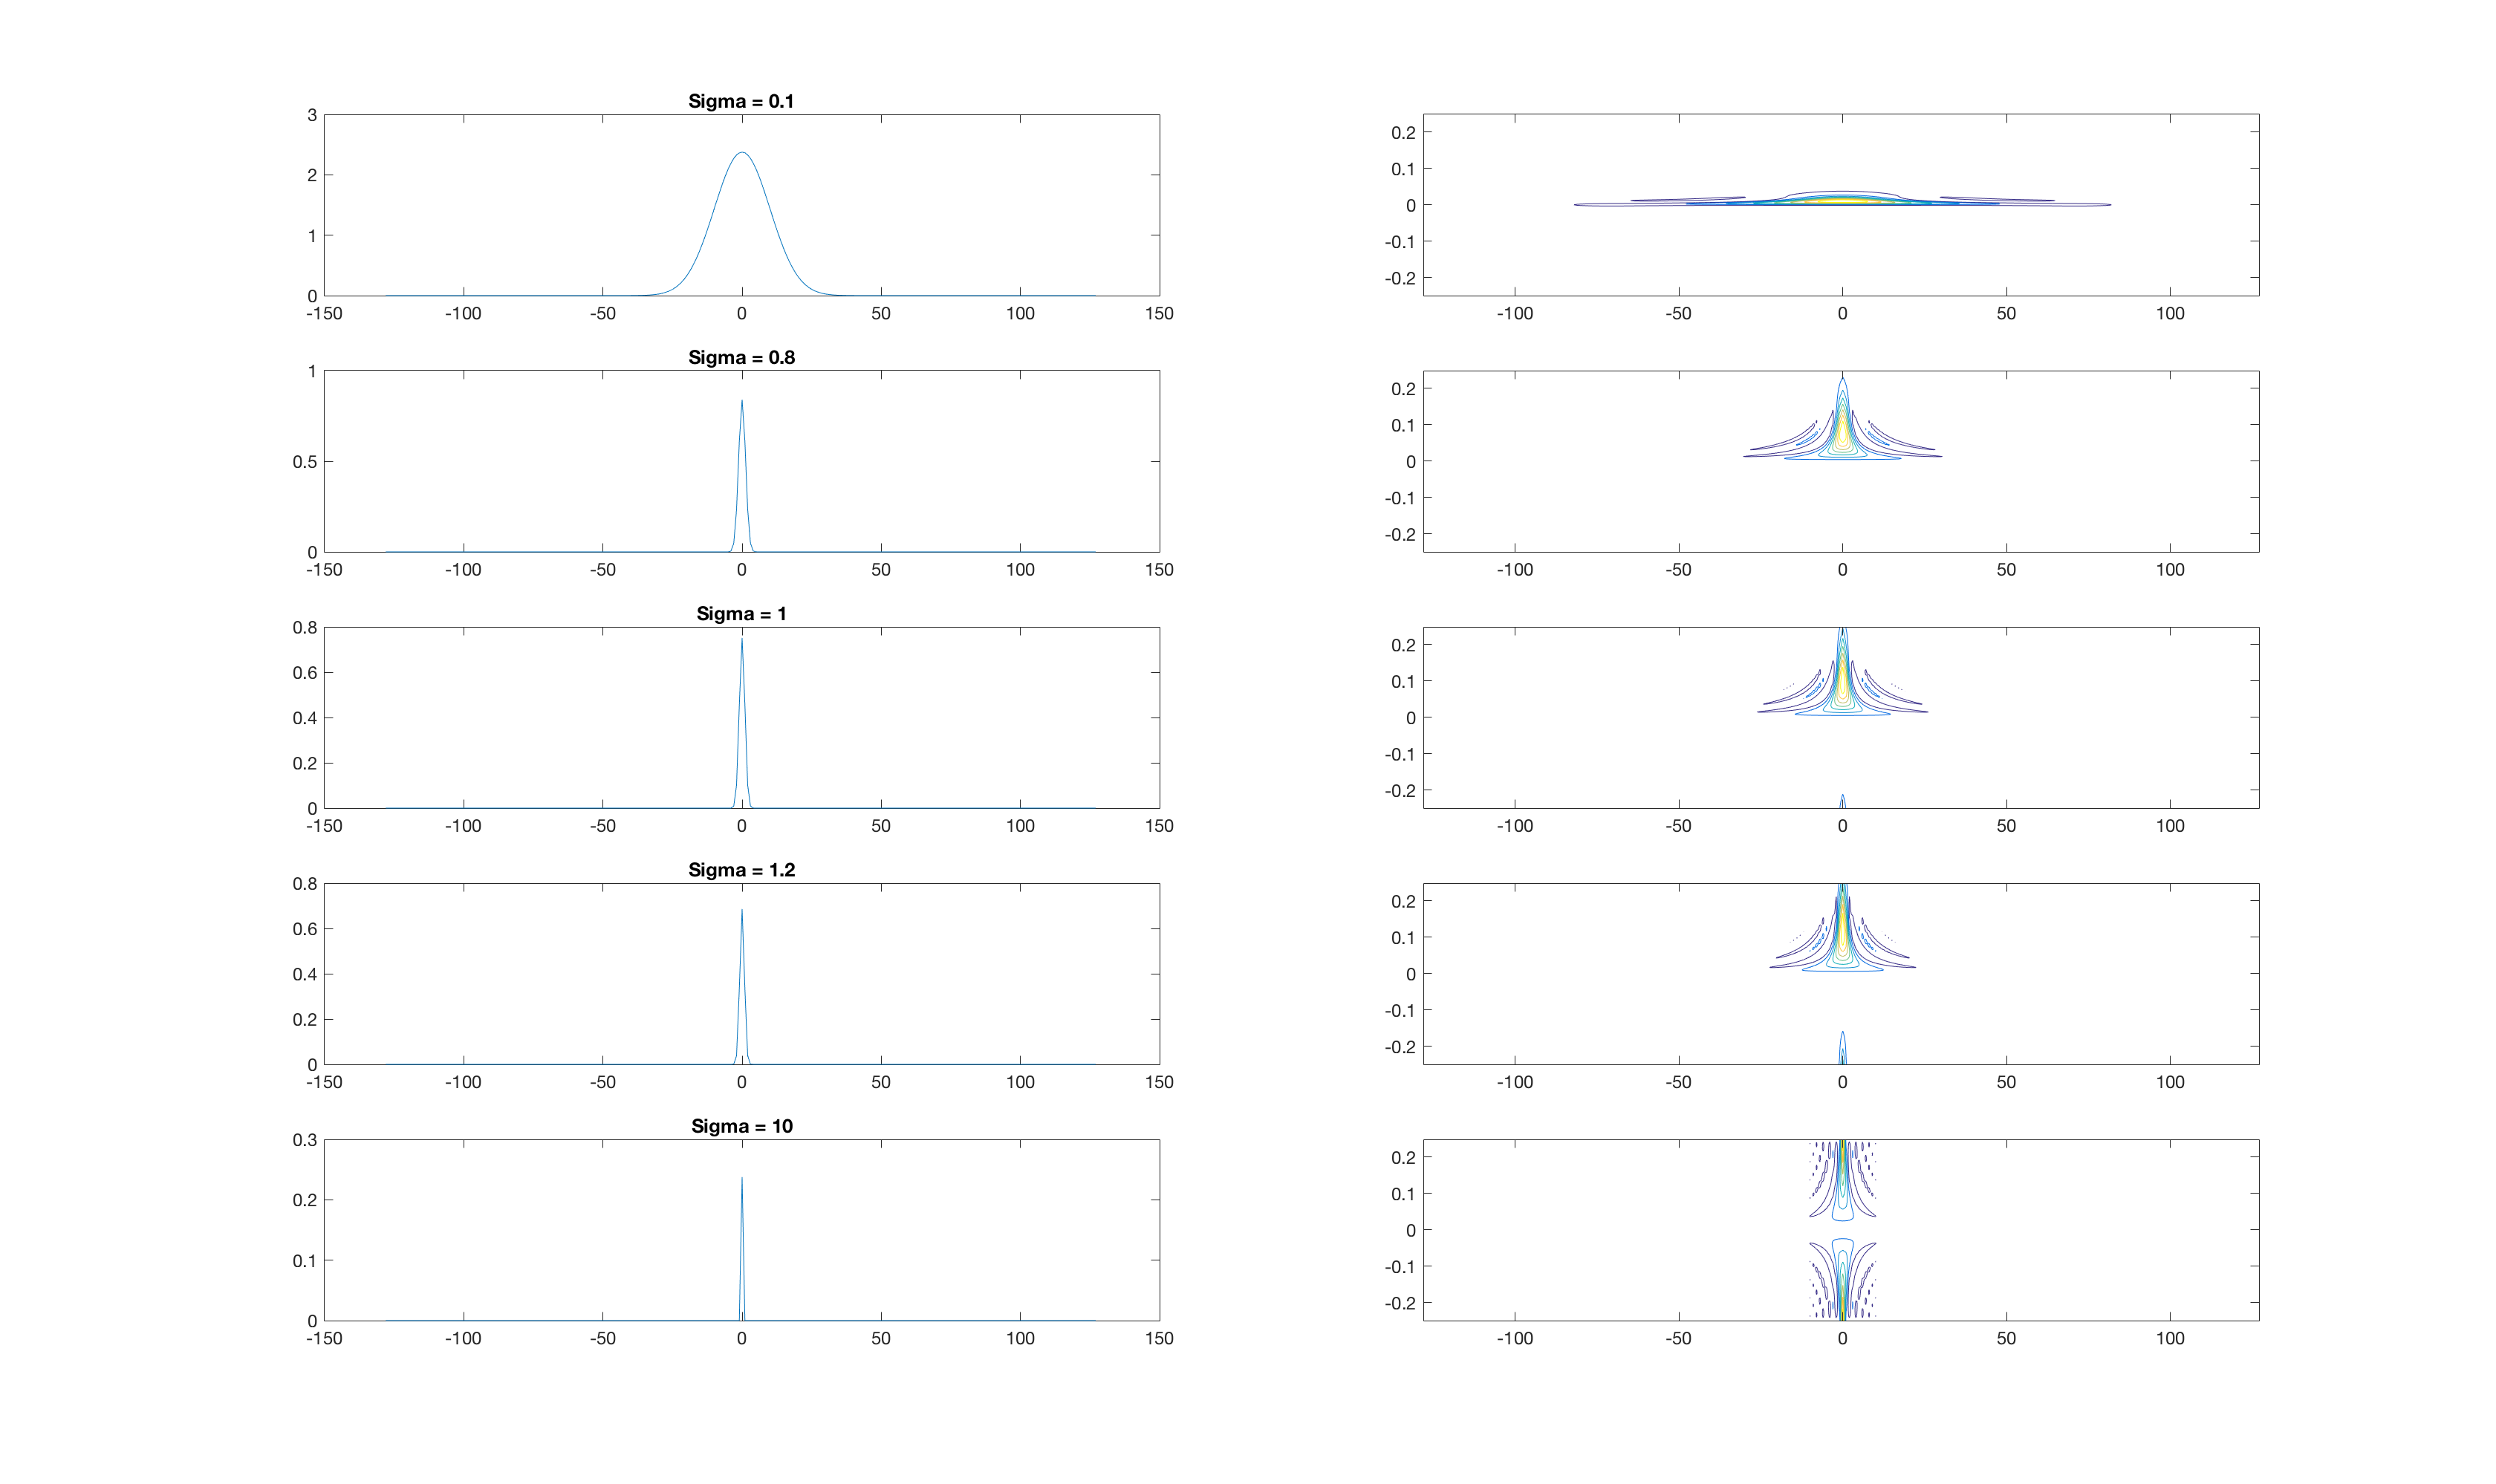
\includegraphics[scale=.15]{Images/WVD_gauss}
\caption{Fig in the left hand side represents the Gaussian function $g(t)$ as defined above for various $\sigma$ values. Fig in the right land side represents the Wigner Ville Distribution $WVD_g$ as defined above. The graph is created using the mywvdgauss.m program attached in the Appendix. $WVD$ values are created by using the HOSA (Higher Order Spectral Analysis) Matlab toolbox. }
\label{fig:WVD_gauss}
\end{figure}

The WVD is time and frequency-shift invariant. Let

\begin{equation}
h(t) = g(t-mT) e^{-jn\Omega t}
\end{equation} where $\Omega$ and $T$ are the frequency and time sampling steps respectively. The WVD of $h(t)$ is given by,

\begin{equation}
WVD_h(t,\omega) = 2e^{-[\frac{(t-mT)^2}{\sigma^2}+[\sigma(\omega-n\Omega)]^2]}
\end{equation}

\begin{equation}
WVD_h(t,\omega) = WVD_g(t-mT,\omega-n\Omega)
\end{equation}

Let $s(t) = h(t)+h'(t)$, then $WVD_s(t,\omega)$ is given as
\begin{equation}
WVD_s(t,\omega) = WVD_h(t,\omega)+WVD_{h'}(t,\omega)+2Re[{WVD_{h,h'}(t,\omega)}]
\end{equation}

where $WVD_{h,h'}(t,\omega)$ is given by
\begin{equation}
 WVD_{h,h'}(t,\omega) = e^{j\omega_d t_\mu} H(t-t_\mu, \omega-\omega_\mu)
\end{equation}

where
\begin{equation}
H(t,\omega) = 2e^{-[\frac{t^2}{\sigma^2}+(\sigma \omega)^2]} e^{-j[t_d\omega - \omega_dt]}
\end{equation}

\begin{equation}
\begin{aligned}
t_\mu &= \frac{m+m'}{2} T  \\
\omega_\mu &= \frac{n+n'}{2}\Omega \\
t_d &= (m - m')T \\
\omega_d &= (n-n')\Omega 
\end{aligned}
\end{equation}

The $WVD_{h,h'}(t,\omega)$ has the same envelope as the $WVD_g(t,\omega)$ but is oscillating with frequency $\omega_d$ in the time domain and $t_d$ in the frequency domain. The location of $WVD_{h,h'}(t-t_\mu,\omega-\omega_\mu)$ is halfway between $h$ and $h'$. The $2Re$[$WVD_{h,h'}(t,\omega)$] is the cross term. When a signal $s(t)$ can be decomposed as a linear combination of some elementary functions $h(t)$ then the cross-terms can be controlled. 

Recall from the previous chapter on the Gabor Expansion, for a given signal $s(t)$, the orthogonal-like Gabor expansion is defined as follows. 

\begin{equation}
s(t) = \frac{1}{\sqrt{2\pi}} \sum_{m=-\infty}^{\infty} \sum_{n=-\infty}^{\infty} C_{m,n} g(t-mT) e^{jn\Omega t}
\end{equation}

The Gabor coefficients $C_{m,n}$ are determined by

\begin{equation}
C_{m,n} = \int s(t) \gamma^{*}_{m,n}(t) dt = \int s(t) \gamma^{*}(t-mT)e^{-jn\Omega t} dt = STFT(mT,n\Omega)
\end{equation}

Using the Wigner-Ville distribution of $s(t)$ from the above equation yields,

\begin{equation}
WVD_s(t,\omega) = \sum_{m,n} \sum_{m',n'} C_{m,n} C_{m',n'} WVD_{h,h'}(t,\omega)
\end{equation}

where


\begin{equation}
 WVD_{h,h'}(t,\omega) = e^{j\omega_d t_\mu} 2e^{-[\frac{(t-t_mu)^2}{\sigma^2}+(\sigma (\omega-\omega_\mu))^2]} e^{-j[t_d\omega - \omega_d t]}
\end{equation}

\begin{equation}
WVD_s(t,\omega) = \sum_{m,n} \sum_{m',n'} C_{m,n} C_{m',n'} e^{j\omega_d t_\mu} 2e^{-[\frac{t^2}{\sigma^2}+(\sigma \omega)^2]} e^{-j[t_d\omega - \omega_dt]}
\end{equation}

where $t_d$ and $\omega_d$ reflect the degree of oscillation. 

When $m=m'$ and $n=n'$, 
\begin{equation}
C_{m,n} C^*_{m',n'} WVD_{h,h'}(t,\omega) = 2|C_{m,n}|^2 e^{-[\frac{(t-mT)^2}{\sigma^2}+\sigma^2 (\omega-n\Omega)^2)]} 
\end{equation}

When $m\neq m'$ or $n \neq n'$

\begin{equation}
C_{m,n} C^*_{m',n'} WVD_{h,h'}(t,\omega) = C_{m,n}C^{*}_{m',n'} e^{j\omega_d t_\mu} H(t-t_\mu,\omega-\omega_\mu)
\end{equation}

Based on the decomposition of the Wigner-Ville distribution defined above, the Time Frequency Distribution Series (TFDS) is defined as follows. 

\begin{equation}
TFDS_D(t,\omega) = \sum_{d=0}^{D} P_d(t,\omega)
\end{equation}

Here $P_d(t,\omega)$ is the sum of a sequence of $WVD_{h,h'}(t,\omega)$ which have a similar contribution to the useful properties and similar influence to the cross terms in which $|m-m'|+|n-n'|=d$

\begin{equation}
P_d(t,\omega) = \sum_{|m-m'|+|n-n'|=d} C_{m,n}C^{*}_{m',n'} WVD_{h,h'}(t,\omega)
\end{equation}

Substituting the value of $WVD_{h,h'}(t,\omega)$ in the above equation, we get

\begin{equation}
P_d(t,\omega) = \sum_{|m-m'|+|n-n'|=d} C_{m,n}C^{*}_{m',n'} e^{j\omega_d t_\mu} 2e^{-[\frac{t^2}{\sigma^2}+(\sigma \omega)^2]} e^{-j[t_d\omega - \omega_d t]}
\end{equation}

Substituting the value of $t_d$, $\omega_d$, $t_\mu$ and $\omega_\mu$, we get

\begin{equation}
P_d(t,\omega) = \sum_{|m-m'|+|n-n'|=d} C_{m,n}C^{*}_{m',n'} e^{j\frac{n+n'}{2}\Omega(m-m')T} 2e^{-[\frac{t^2}{\sigma^2}+(\sigma \omega)^2]} e^{-j[(m-m')T\omega - (n-n')\Omega t]}
\end{equation}

Both the SP500 and NASDAQ indices are discrete signals used for analysis. The $P_d$ is further simplified for programming convenience. 

The discrete Time Frequency Distribution Series is defined as follows. 

\begin{equation}
DTFDS_D[i,k] = TFDS_d(t,\omega) |_{ t = i\Delta t, \omega = \frac{2\pi k}{L\Delta t}}
\end{equation}
for $-\frac{L}{2} \leq k < \frac{L}{2}$ where $\frac{1}{\Delta t}$ denotes the sampling frequency. $L$ denotes the length of the signal. The discrete time frequency distribution series can be summarized as 

\begin{equation}
 TFDS_d(i,k) = \sum_{d=0}^{D} P_d[i,k]
\end{equation}

where 
\begin{equation}
 P_d[i,k] = \sum_{|m-m'|+|n-n'|=d} C_{m,n}C_{m'n'} WVD_{h,h'}[i,k]
\end{equation}

The $TFDS_D[i,k]$ is the sum of all $WVD_{h,h'}[i,k]$ in which the distance of the corresponding Gabor elementary functions $h_{m,n}[i]$ and $h_{m',n'}[i]$ is less than or equal to d. $WVD[i,k]$ is defined as a sampled Wigner-Ville distribution. 

\begin{equation}
WVD_s[i,k] = WVD_s(t,\omega) |_{ t=i\Delta t, \omega = \frac{2\pi k}{L\Delta t}}
\end{equation}
where $\Delta t$ denotes the sampling interval. For the Gaussian functions, WVD is obtained by sampling the formula. 

\begin{equation} \label{eq:1}
WVD_{h,h'}[i,k] = 2e^{-\sigma(i-\frac{m+m'}{2}\Delta M)^2-\frac{1}{\sigma}(k-\frac{n+n'}{2}\Delta N)^2} e^{j\frac{2\pi}{L}[(m-m')\Delta M k +(n-n')\Delta Ni - \frac{n+n'}{2}\Delta N(m-m')\Delta M]}
\end{equation}

We assume $\Delta t =1$. $WVD_{h,h'}[i,k]$ in \ref{eq:1} is completely determined by the parameters of the Gabor expansion, such as $\Delta M, \Delta N, L$ and $\sigma$ which are independent of the analyzed signal. Therefore, once $\Delta M, \Delta N, L$ and $\sigma$ are determined, $WVD_{h,h'}[i,k]$ can be precomputed and saved in a table. 
